\chapter{Application Analysis} \label{ch:appanalysis}
\todo{ikke færdig}
This chapter starts by describes the basic principles of stereo vision then different aspects such as color versus gray scale etc are analyzed. 

\section{basic principal of stereo vision}\label{sec:basicstereo}
A stereo vision setup normally consists of two cameras placed horizontally at a specified distance from each other (the baseline). An example of this is on figure \ref{fig:2cams_all}


\begin{figure}[ht]
  \centering
  \begin{subfigure}[t]{1\textwidth}
    \centering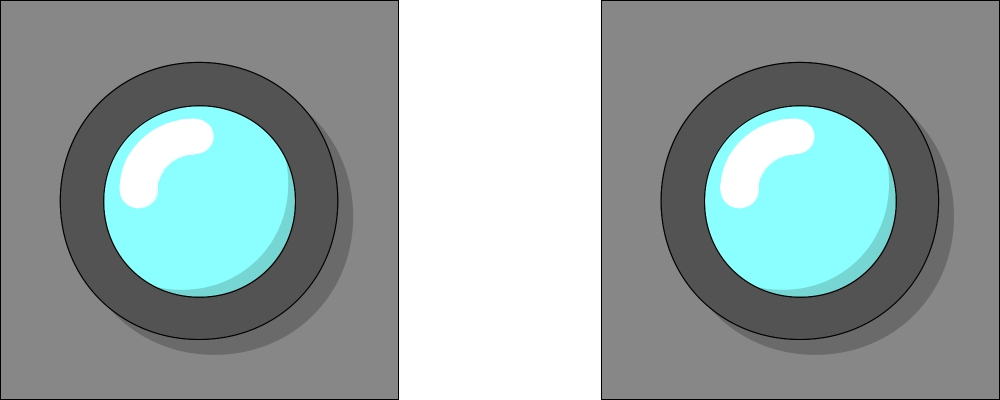
\includegraphics[width=0.5\textwidth]{figures/2cams_fro}
    \caption{Seen from the front\label{fig:2cams_fro}}
  \end{subfigure}\vspace{0.5cm}
  \begin{subfigure}[t]{1\textwidth}
    \centering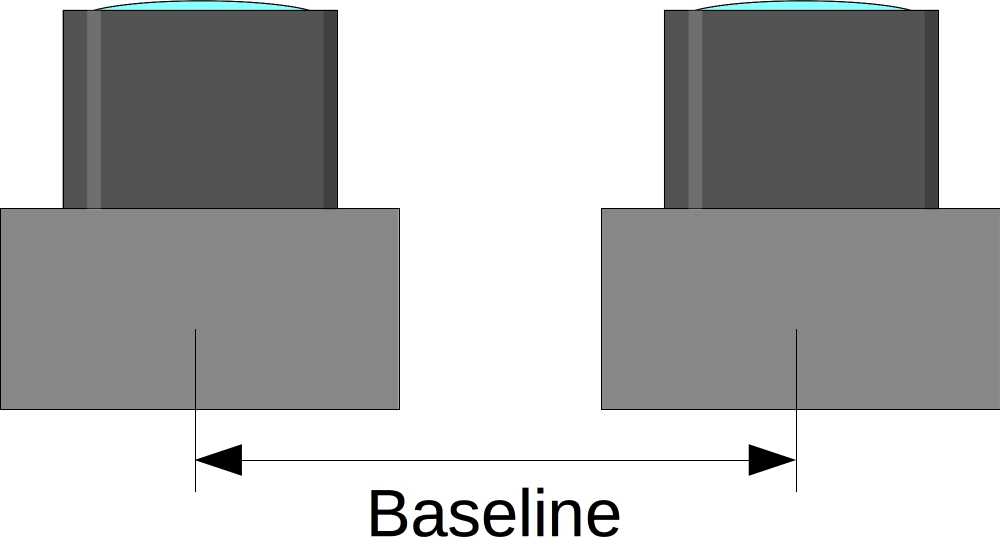
\includegraphics[width=0.5\textwidth]{figures/2cams_top}
    \caption{Seen from above\label{fig:2cams_top}}
  \end{subfigure}
  \caption{Illustration of stereo setup\label{fig:2cams_all}}
\end{figure}

Figure \ref{fig:imgplane_all} shows how a scene is seen by the camera, is inverted in the optical center and projected onto the image sensor in the camera. The original image plane is located at the position of the image sensor but it is inverted compared to scene captured. To simplified comparisons to the real world an image plane can be placed opposite of the optical center at the same distance from the center and this image plane will not be inverted.  

\begin{figure}[ht]
  \centering
  \begin{subfigure}[t]{0.3\textwidth}
    \centering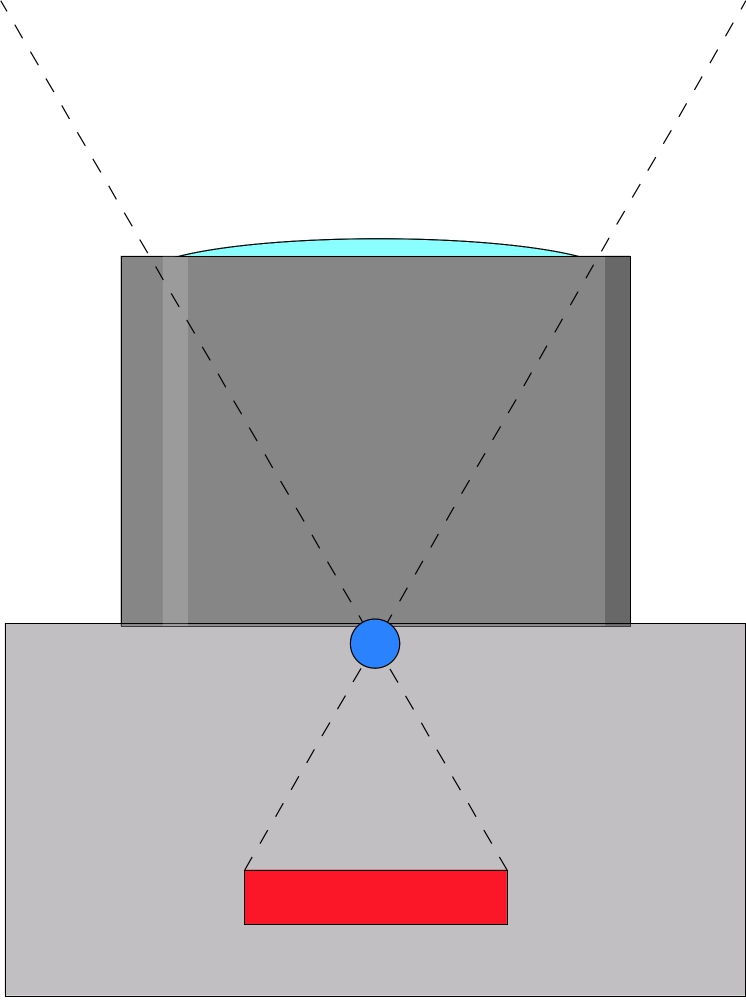
\includegraphics[height=4cm]{figures/imgplane_1.jpg}
    \caption{Location of the optical center and image sensor\label{fig:imgplane1}}
  \end{subfigure}\hspace{0.5cm}
  \begin{subfigure}[t]{0.3\textwidth}
    \centering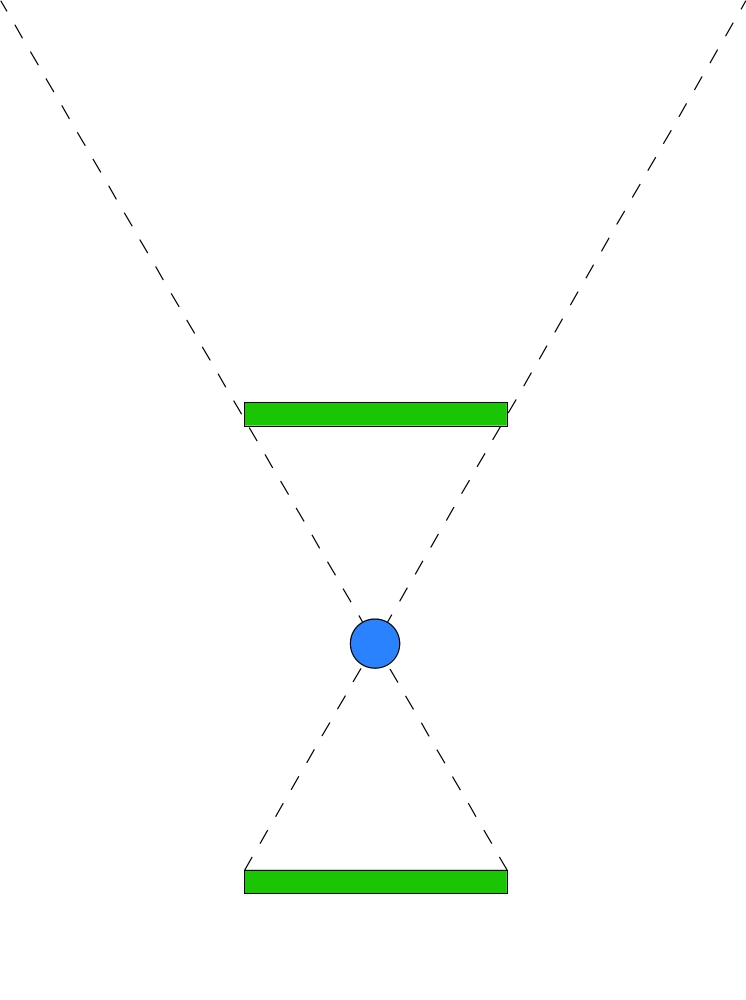
\includegraphics[height=4cm]{figures/imgplane_2}
    \caption{Location of the image plane\label{fig:imgplane2}}
  \end{subfigure}\hspace{0.5cm}
  \begin{subfigure}[t]{0.3\textwidth}
    \centering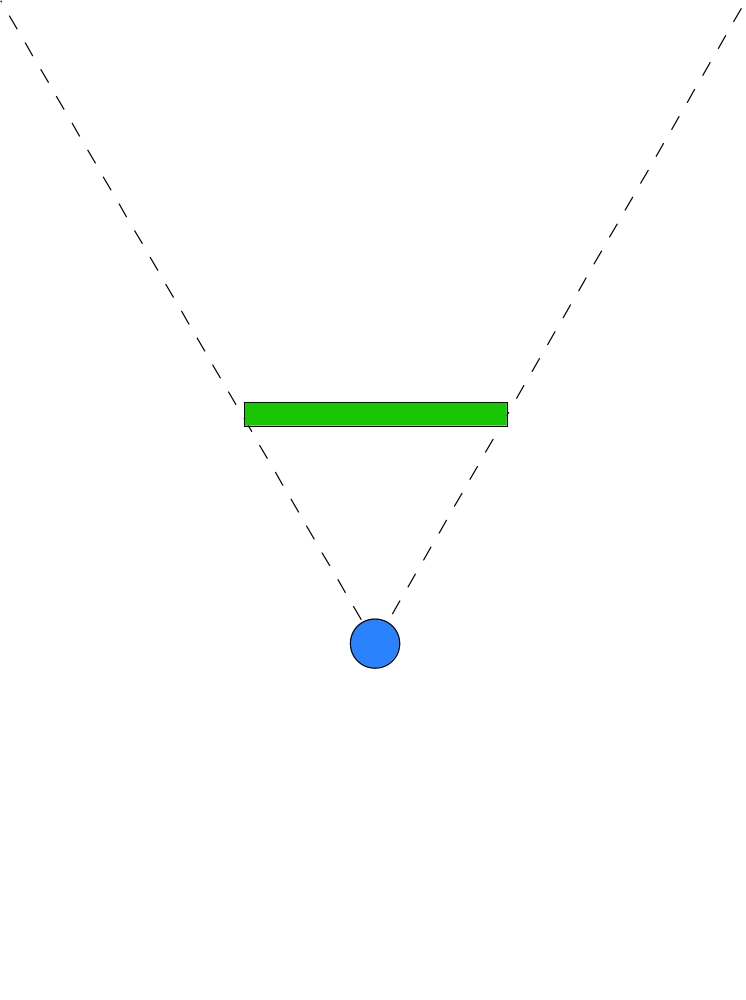
\includegraphics[height=4cm]{figures/imgplane_3}
    \caption{This illustration will be used to to explain disparity\label{fig:imgplane3}}
  \end{subfigure}
  \begin{subfigure}[t]{0.75\textwidth}
    \centering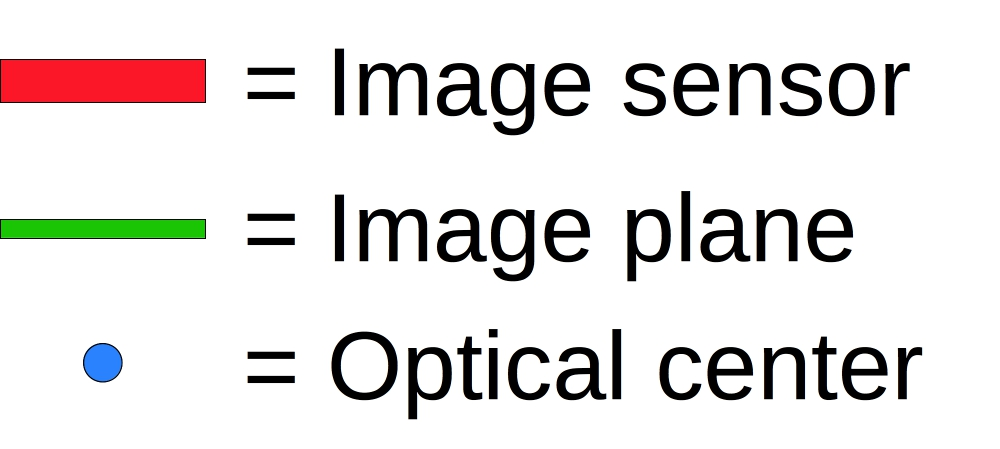
\includegraphics[width=0.4\textwidth]{figures/imgplane_legends}
  \end{subfigure}\hspace{0.5cm}
  \caption{Illustration of going from camera to image plane\label{fig:imgplane_all}}
\end{figure}

Figure \ref{fig:2points_1} shows that a single camera is not able to differentiate between two points at the same angle from the optical center but a different distance. Figure \ref{fig:2points_2} shows that adding the second camera shows that you then are able to differentiate between the two points.

\begin{figure}[ht]
  \centering
  \begin{subfigure}[t]{0.45\textwidth}
    \centering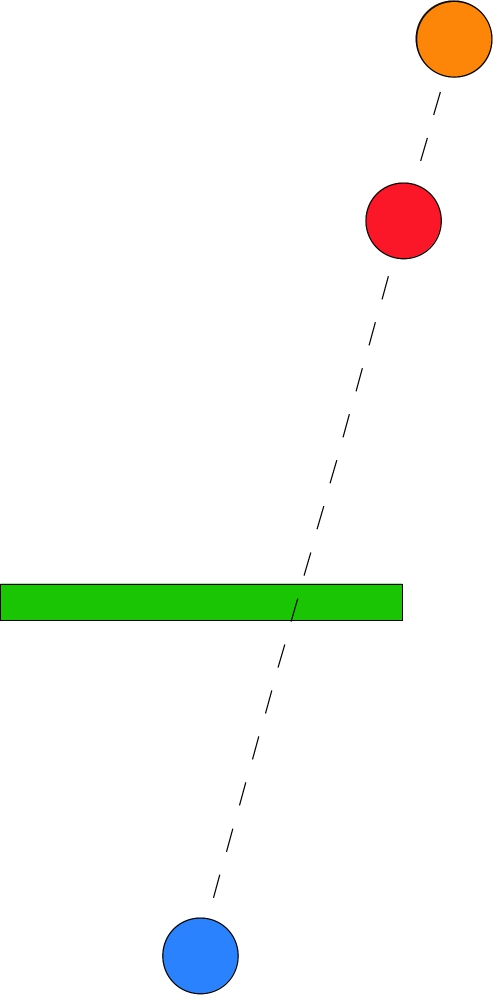
\includegraphics[height=4cm]{figures/2points_1}
    \caption{Seen from a single camera\label{fig:2points_1}}
  \end{subfigure}
  \begin{subfigure}[t]{0.45\textwidth}
    \centering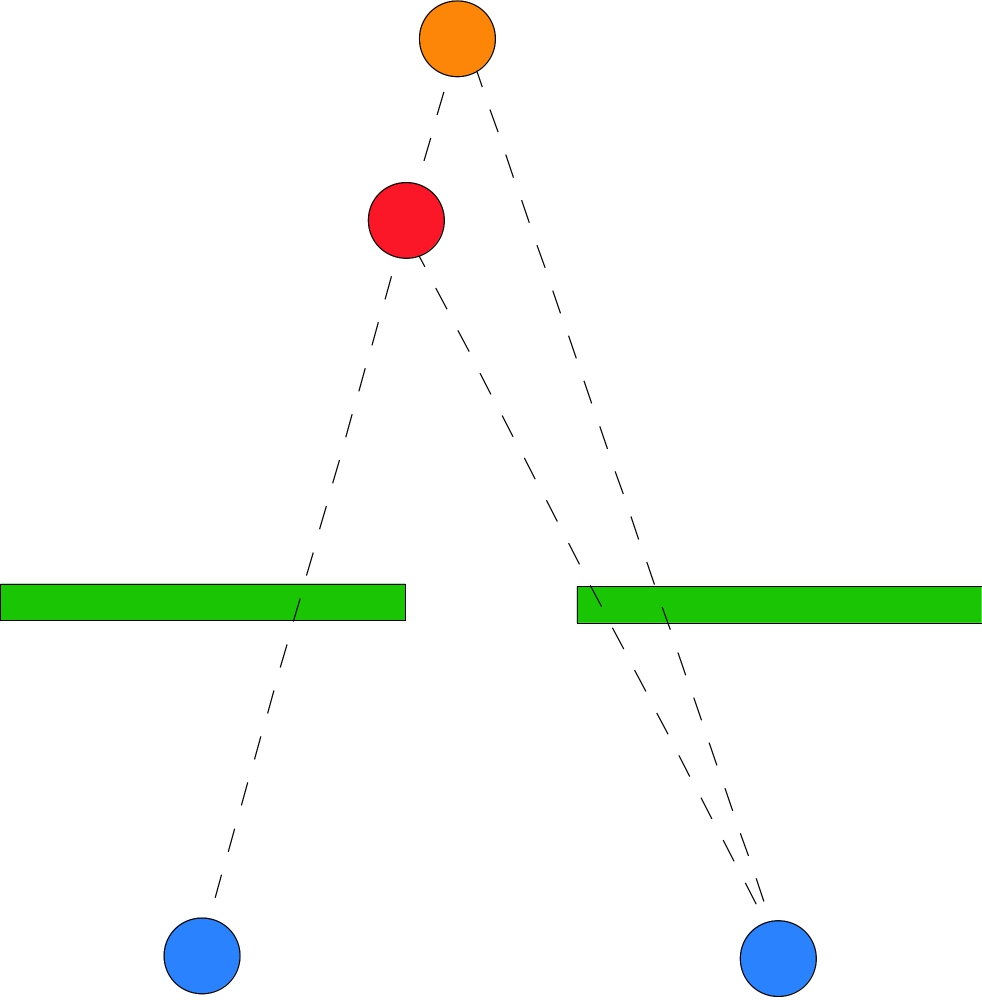
\includegraphics[height=4cm]{figures/2points_2}
    \caption{Seen from two cameras\label{fig:2points_2}}
  \end{subfigure}
  \caption{Example pf two points in a scene at different depths\label{fig:2points_all}}
\end{figure}

Figure \ref{fig:dispall} shows how the depth to a point can be calculated from the difference in x-positions on the image plane (the disparity). Figure \ref{fig:disp_long} and \ref{fig:disp_short} shows how the disparity change depending on the distance to the point. Two similar triangles can be created. One between the point, and the two optical centers. The other triangle is created between the point in the scene and the points where the dashed lines cross the image plane. Figure \ref{fig:bfz_disp} shows these two triangles and their heights. The small triangle have a height of $z$ and the bottom (the brown line) is equal to the baseline (purple line) minus the disparity and the large triangle have a height of $f+z$ and the bottom width is equal to the baseline. The ratio between the height and the bottom width is the same in the two triangles and hence the following equation can be formed:
\begin{flalign}
  && \frac{z+f}{b} &= \frac{z}{b-d} && \label{eq:disp_1} \\
  && z &= \frac{b \cdot f}{d} && \label{eq:disp_final}
\end{flalign}
\todo{ret denne formel til på et tidspunkt. \ref{eq:disp_final} er korrekt. Ændre den anden + måske figuren (z går vist fra baseline og ikke bare fra image plane)}

\begin{figure}[ht]
  \centering
  \begin{subfigure}[t]{0.3\textwidth}
    \centering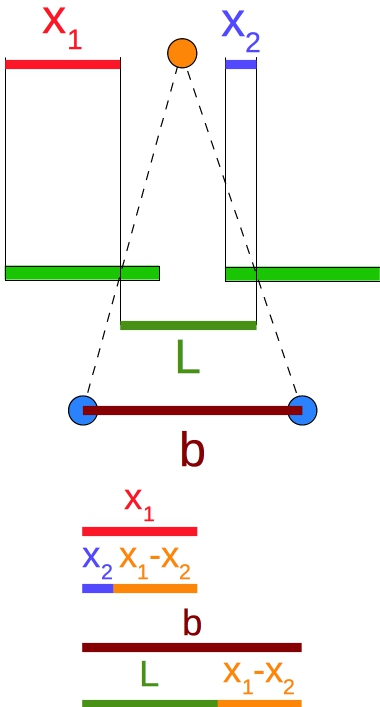
\includegraphics[height=5cm]{figures/disp_long.jpg}
    \caption{Disparity for a point far way\label{fig:disp_long}}
  \end{subfigure}\hspace{0.5cm}
  \begin{subfigure}[t]{0.3\textwidth}
    \centering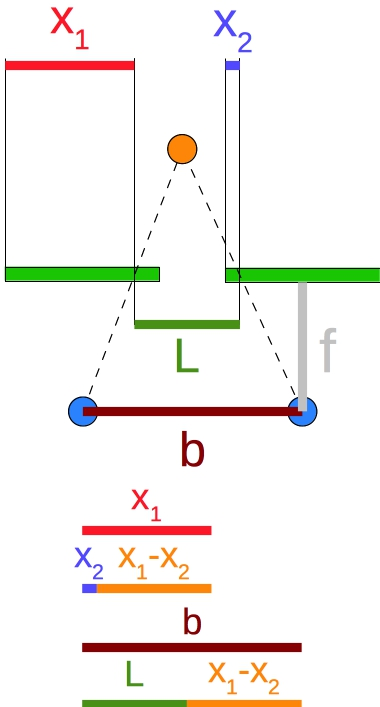
\includegraphics[height=5cm]{figures/disp_short}
    \caption{Disparity for point close\label{fig:disp_short}}
  \end{subfigure}\hspace{0.5cm}
  \begin{subfigure}[t]{0.3\textwidth}
    \centering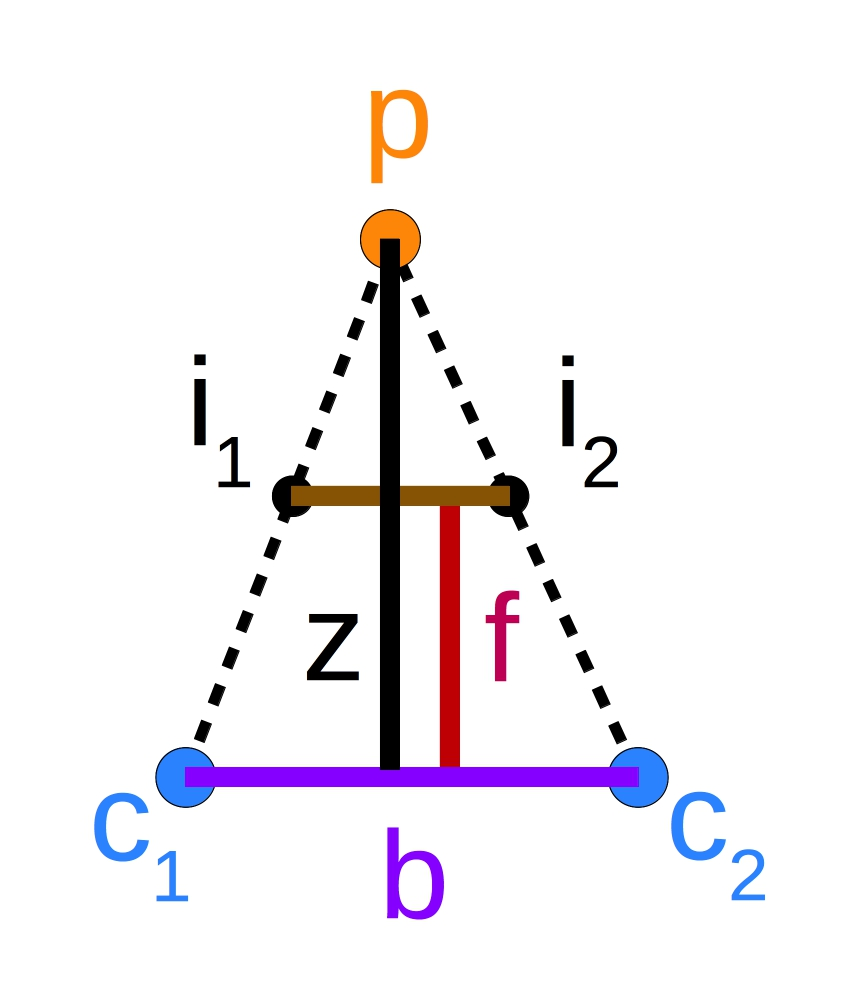
\includegraphics[height=5cm]{figures/bfz_disp}
    \caption{Illustration of triangles used for calculating the disparity\label{fig:bfz_disp}}
  \end{subfigure}
  \caption{Illustration of how to calculate depth from disparity\label{fig:dispall}}
\end{figure}

This explains the basic of stereo vision. The rest of this chapter will venture into other areals of stereo and describe the difficulties and solutions for each area.

\section{Rectification of stereo pairs}
The examples in section \ref{sec:basicstereo} uses ideal images to explain how stereo vision functions but in the real world the disparity is the difference along the epipolar lines which will have a different slope of each line and image. Different things can be done to simplify the search along epipolar lines. One thing is to rectify the stereo image pair. This will make all the epipolar lines horizontal and hence you only need to search along the x-axis.\\

The issue with rectification is that it is difficult to get a perfect match with the stereo setup since the every camera and its objective will be unique and require and all new manual adjustment. HSA system theorizes that a system can be developed which instead of rectifying the image it will find the epipolar lines and feed this information to the stereo camera. In this project stereo image pairs from Middlebury Vision Test set \cite{da} will be used which are rectified hence the rectification of image will not be researched further in this project.

\section{Color space and gray scale}
\todo{skriv noget om forskellige farve rum og grayscale og deres inflydelse på stereo algorithmen}
The article \textbf{Color correlation-based matching} takes the subject of difference in result when using color and which color space is used and grayscale when performing stereo matching. It performs different methods / algorithms using 9 different colorspace including grayscale. The result from the article is that color gives a better result with a few percentage of more correct estimations but the run time is much higher (ranging from 1.9 to 3.7 higher run time than grayscale on the teddy test set).
From this it is decided to not use color in case of Normalized Cross Correlation

\section{Resolution and disparity precision}
\todo{skriv noget om disparitets opløsning i forhold til billede opløsning osv.}

\section{Occlusion filling}
\todo{skriv noget om metoder til at udfylde occlusions områder}
This section will describe methods for filling the occluded areas. All these methods comes from the article: \textit{Occlusion filling in stereo: Theory and experiments} by \textit{Shafik Hyq, Andreas Koschan} and \textit{Mongi Abidi}. All these methods assume that the stereo matching is going from left image to right image i.e. templates are taken from the left image matched onto the right image.
 
\subsection{Neighbor's Disparity Assignment : NDA}
This is the simplest method to fill occlusions. It functions by selecting an occluded point, $p_L$, then find then nearest non-occluded point, $q_L$, to the left when filling non-border occlusion. With border occlusion the nearest point to the right is found instead. It is assumed that this non-occluded point is part of same surface as the occluded point (this can be seen on figure \ref{fig:borNParOcc}) and the disparity value from $q_L$ can be assigned to $p_L$. This method have some issues. In cases of total occlusions (see figure \ref{fig:totalOcc}) then a wrong disparity value is given to the total occluded object since it isn't a part of the nearest surface with non-occluded points to the left. In cases with self occlusions the occluded area should have disparity values close to the disparity values of the non-occluded points to the right (This will be the area of the surface which is in view of both cameras) but using NDA will give the occluded area disparity values corresponding to the background. 

\subsection{Diffusion in Intensity Space : DIS}
This method is inspired by diffusion. Diffusion is the movement of molecules or atoms from a high concentration region to a low concentration region. \\
After detecting occluded regions with cross-checking during template matching, the diffusion energy for the region is approximated. This method is depended on the stereo matching algorithm because it use the energy from the last iteration to determine initial diffusion energy for the area. \\
A change to the method can be made to make it independent from the stereo matching. The initial energy will be 0. Then the diffusion energy for non-border occlusion is found by:
\begin{equation}
E(p_L) = \min_{l_{p_L}=\{0,\dots, l_{max}\}} \left( \dfrac{1}{2 | q_L \in \mathcal{N}(p_L) \wedge l_{q_L=l_{p_L}} |} \; \sum_{q_L \in \mathcal{N}(p_L) \wedge l_{q_L = l_{p_L}}} (|\bar{I}(p_L)-\bar{I}(q_L) | + E(q_L))\right)
\end{equation}
And the diffusion energy for border occlusions are found by by:
\begin{equation}
E(p_L) = \min_{l_{p_L}=\{0,\dots, l_{p_{Lf}}-2\}} \left( \dfrac{1}{2 | q_L \in \mathcal{N}(p_L) \wedge l_{q_L=l_{p_L}} |} \; \sum_{q_L \in \mathcal{N}(p_L) \wedge l_{q_L = l_{p_L}}} (|\bar{I}(p_L)-\bar{I}(q_L) | + E(q_L))\right)
\end{equation}
The diffusion energy will be calculated for each occluded point and for each point the disparity which corresponds the minimum $E(p_L)$ is set as the disparity $l_{p_L}$ for the occluded point. 


\subsection{Weighted Least Squares : WLS}
In this approach, WLS, all the non-occluded and filled occluded neighbors in a neighborhood around the occluded point is considered valid points and is used as control points in interpolation.\\
Since the neighborhood contains both foreground points and background points and the occluded point is expected to be a part of the background then the background points should have more influence than foreground points. It is assumed that the color intensity between objects is significantly different and this property can be used to distinguish between foreground points and background points. \\
Each error term in the aggregated residual should be weighted so the foreground don't have much influence. With this the aggregated residual is defined as:
\begin{equation}
  \Delta = \sum_{q_L \in \mathcal{N}(p_L)} w_{q_L} (\hat{l}_{p_L}(p_L)-l_{p_L}(q_L))^2
\end{equation}
where $w_{q_L} = e^{-\mu_L | \bar{I}(p_L) - I(q_L)|}$ (the weight) is the likelihood of $p_L$ with $q_L$ under the assumption of an exponential distribution model of $| \bar{I}_(p_L)- I(q_L) |$. $\bar{I}(p_L)$ is the mean intensity of $p_L$ and $\mu_L$ is the decay rate. $\hat{l}_{p_L}(p_L)$ is the estimated disparity of $p_L$ (will be estimated during interpolation) and $l_{p_L}(q_L)$ is the disparity of $q_L$. \\
How to estimate $\bar{I}(p_L)$ and $\mu_L$:\\
$\bar{I}(p_L)$ is the mean intensity of $p_L$ which can be obtained using mean shift algorithm in a window around $p_L$. To estimate this value the initialize the algorithm with $\bar{I}(p_L) $ equal to the intensity of $p_L$ then the mean shift algorithm repeatedly picks those neighbors inside the window that satisfy $| \bar{I}(p_L) - I (q_L) | \geq 3\mu^{-1}$ and the assign the average of intensities of the selected neighbors to $\bar{I}(p_L)$ until $\bar{I}(p_L)$ converges to a fixed average. $|\bar{I}(p_L) - I(q_L)|$ has decay rate $\mu_L$ which is related to the decay rate $\mu$ of the variable $|I(p_L) - I(q_L)|$ by $\mu_L^2 = \mu$.\\
A matrix containing all the coordinates:
\begin{equation}
F = \begin{bmatrix}
  x_1 & y_1 & 1 \\
  \vdots & \ddots & \vdots\\
  x_n & y_n & 1 
\end{bmatrix}
\end{equation}
Vector with the corresponding labels for the coordinates in $F$:
\begin{equation}
L = [l_1 \; \cdots \; l_N] 
\end{equation}
Linear model:
\begin{equation}
l_{p_L} = a + b x (p_L) + c y (p_L)
\end{equation}
Where $(x(p_L),y(p_L))$ is the coordinates of $p_L$ and $a$, $b$ and $c$ are the model parameters. \\
The weights for the control points can be express in a vector as:
\begin{equation}
w = [w_{q_{L1}} \; w_{q_{L2}} \; \cdots \; w_{q_{LN}}]'
\end{equation}
Then we compute two new matrices, $F_w$ and $L_w$:
\begin{flalign}
&& F_w &= diag(w)F && \\
&& L_w &= diga(w)L &&   
\end{flalign}
The model parameter vector:
\begin{equation}\label{eq:parvec}
P = [\, a \; b \; c \,]'
\end{equation}
By combining the equations above then the following equation is given: 
\begin{equation}
P = (F^T_wF_w)^{-1}F^T_wL_w
\end{equation}
With these equation the disparity of the occluded point can be estimated:
\begin{equation}
\hat{l}_{p_L} = [1 \; x(p_L) \; y(p_L)] P
\end{equation}

\subsection{Segmentation-based Least Squares : SLS}
Biggest difference between WLS and SLS is that SLS only uses non-occluded points as control points. The control points is a subset of the non-occluded neighboring points. The control points are segmented from the neighborhood by applying different constraints: visibility constraint, disparity gradient constraint and color similarity cues. \\
Sequence of operations: 
\begin{itemize}
\item Select an occluded point
\item Select control points from the neighborhood around the occluded point
\item Interpolate the disparity of the occluded point from the segmented control points 
\end{itemize}
$\mathcal{N}(p_L)$ is a set of non-occluded, neighboring points which will be use for control points in the interpolation. For points to be added to $\mathcal{N}$ then it needs to fulfill some constraints.\\
\textbf{Disparity gradient constraint:} In most cases the horizontal closest non-occluded point to the right, $p_{Lf}$, will be part of the foreground and the occluded should be a part of the background. In this cases every non-occluded point with a lower disparity than $p_{Lf}$ will be added to $\mathcal{N}$ hence the condition for added the point, $q_L$, will be $l_{q_L} < l_{p_{Lf}}$. If the foreground object is narrow then all the non-occluded neighboring points might be from the background and have the same disparity. Due to this a second condition have to be added to the constraint. The horizontal closest non-occluded point to the left will be called $p_{Lb}$ and a second condition is created: $| l_{p_{Lb}} - l_{q_L} | \leq 1$. When these conditions are combined the constraint can be defined as:
\begin{equation}
| l_{p_{Lb}} - l_{q_L} | \leq 1 \vee  l_{q_L} < l_{p_{Lf}}  
\end{equation}
\textbf{surface constraint:} It is assumed that $\mathcal{N}(p_L)$ will contain points from maximum 2 different surfaces (due to the small neighborhood). Some cases might contain a third surface but this is expected to occur very seldom and therefore it is disregarded. The point with the lowest disparity, $l_{min}$, is assumed to belong to one of the surfaces and the point with the highest disparity, $l_{max}$, is assumed to belong to the other surfaces. If $l_{max} - l_{min} \leq 1$ then it is assumed the all the points in $\mathcal{N}$ belongs to a single surfaces otherwise the points have to be segmented into 2 groups. The first group will contain all points which satisfies $| l-{max} - l_{q_L} | \leq 1$ and the other group will contain all the points which satisfies $| l-{min} - l_{q_L} | \leq 1$.
\textbf{Color constraint:} The average truncated color distance from the occluded point, $p_L$, to each of the two groups to determine which group the point belongs to. The average truncated color distance is found by:
\begin{equation}
D(p_L,\mathcal{N}_i(p_L) ) = \dfrac{1}{|\mathcal{N}_i(p_L)|} \; \sum_{q_L \in \mathcal{N}(p_L)} \psi (p_L,q_L) 
\end{equation}

\section{Mini-conclusion}
\todo{find på et bedre navn til denne sektion}
To conclude this chapter the findings for each area in stereo vision will be examined and it will be specified which solution will be used from this point.
\subsection*{•}